\documentclass[10pt,twocolumn,letterpaper]{article}

% ============================================================================
% Packages — Nature Communications / JCIM Publication-Grade Typography
% ============================================================================
\usepackage[utf8]{inputenc}
\usepackage[T1]{fontenc}
\usepackage[margin=0.72in,top=0.80in,bottom=0.82in,columnsep=0.25in]{geometry}
\usepackage{mathpazo}           % Palatino serif + matching math
\usepackage[scaled=0.88]{helvet}
\usepackage{courier}            % Crisp monospace for SMILES/code
\usepackage{microtype}          % Optical margin alignment & font expansion
\usepackage{amsmath,amssymb,amsthm}
\usepackage{mathtools}
\usepackage{graphicx}
\usepackage{booktabs}
\usepackage{tabularx}
\usepackage{multirow}
\usepackage{array}
\usepackage{xcolor}
\usepackage{caption}
\usepackage{subcaption}
\usepackage{fancyhdr}
\usepackage{titlesec}
\usepackage[numbers,sort&compress]{natbib}
\usepackage{hyperref}

% ============================================================================
% Academic Color Palette
% ============================================================================
\definecolor{HarvardCrimson}{HTML}{A51C30}
\definecolor{OxfordNavy}{HTML}{1E3A5F}
\definecolor{BotanicalTeal}{HTML}{0F766E}
\definecolor{WarmOchre}{HTML}{B45309}
\definecolor{InkSlate}{HTML}{0F172A}
\definecolor{MutedSlate}{HTML}{475569}
\definecolor{HairlineGray}{HTML}{CBD5E1}
\definecolor{SoftCanvas}{HTML}{F8FAFC}

\hypersetup{
  colorlinks=true,
  linkcolor=OxfordNavy,
  citecolor=OxfordNavy,
  urlcolor=HarvardCrimson,
  pdftitle={From 3D Protein-Ligand Interactions to Whole-Cell Electrophysiology: Differentiable Multi-Channel Cardiotoxicity Prediction and Closed-Loop Molecular Repair},
  pdfauthor={Jakob Ferschin},
}

% ============================================================================
% Section Headings, Captions & Running Headers
% ============================================================================
\titleformat{\section}
  {\large\bfseries\color{InkSlate}}
  {\thesection.}{0.5em}{}[\vspace{-0.45em}\textcolor{HairlineGray}{\rule{\linewidth}{0.5pt}}]
\titlespacing*{\section}{0pt}{1.05em}{0.45em}

\titleformat{\subsection}
  {\normalsize\bfseries\color{OxfordNavy}}
  {\thesubsection}{0.5em}{}
\titlespacing*{\subsection}{0pt}{0.80em}{0.28em}

\captionsetup{
  font=small,
  labelfont={bf,color=InkSlate},
  textfont={color=InkSlate},
  margin=2pt
}

\pagestyle{fancy}
\setlength{\headheight}{16pt}
\addtolength{\topmargin}{-2pt}
\fancyhf{}
\fancyhead[L]{\scriptsize\sffamily\color{MutedSlate}\textsc{CardioPhys-3D (ADMET-Engine v3.0) — Preprint}}
\fancyhead[R]{\scriptsize\sffamily\color{MutedSlate}\textsc{3D Interactions to Whole-Cell Cardiac Electrophysiology}}
\fancyfoot[C]{\scriptsize\sffamily\color{MutedSlate}\thepage}
\renewcommand{\headrulewidth}{0.4pt}
\renewcommand{\headrule}{\hbox to\headwidth{\color{HarvardCrimson}\leaders\hrule height \headrulewidth\hfill}}

\newtheorem{proposition}{Proposition}

\newcommand{\smiles}[1]{\texttt{\scriptsize #1}}
\newcommand{\qnet}{q_{\mathrm{Net}}}
\newcommand{\pic}{\mathrm{pIC}_{50}}
\newcommand{\cmax}{C_{\max,\mathrm{free}}}
\newcommand{\apd}{\mathrm{APD}_{90}}
\newcommand{\pending}{\textit{Pending A100 run}}

% ============================================================================
% Document Start
% ============================================================================
\begin{document}

% --- Two-column spanning title & abstract block ---
\twocolumn[
\begin{@twocolumnfalse}
  \vspace{-1.4em}
  \noindent\textcolor{HarvardCrimson}{\rule{\linewidth}{2.2pt}}
  \vspace{0.55em}

  \noindent{\scriptsize\sffamily\bfseries\color{HarvardCrimson}\textsc{Research Article \quad $\cdot$ \quad Computational Toxicology \& Biophysical Machine Learning \hfill ADMET-Engine v3.0 (CardioPhys-3D)}}
  \vspace{0.45em}

  \noindent{\LARGE\bfseries\color{InkSlate} From 3D Protein-Ligand Interactions to Whole-Cell Electrophysiology: Differentiable Multi-Channel Cardiotoxicity Prediction and Closed-Loop Molecular Repair}
  \vspace{0.60em}

  \noindent{\normalsize\bfseries\color{InkSlate} Jakob Ferschin\textsuperscript{1}}
  \vspace{0.20em}

  \noindent{\footnotesize\color{MutedSlate}\textsuperscript{1}Independent Researcher, Vienna, Austria \quad $\cdot$ \quad Open-Source Platform \& Release \texttt{v3.0.0}: \href{https://github.com/JakobFerschin/Admet-Engine}{github.com/JakobFerschin/Admet-Engine}}
  \vspace{0.65em}

  \noindent\textcolor{HairlineGray}{\rule{\linewidth}{0.6pt}}
  \vspace{0.35em}

  \begin{quote}
    \small\noindent\textbf{\color{InkSlate}Abstract.}
    Drug-induced Torsades de Pointes (TdP) remains a leading cause of preclinical termination and post-marketing withdrawal. Conventional \textit{in silico} cardiotoxicity models rely on binary 2D quantitative structure--activity relationships (QSAR) targeting only the human ether-\`{a}-go-go-related gene (\textsc{hERG}/K\textsubscript{v}11.1, $I_{\mathrm{Kr}}$) potassium channel. This single-channel paradigm induces systematic false positives for clinically safe multi-channel blockers such as \textbf{Verapamil} and \textbf{Ranolazine}, whose inward L-type calcium ($I_{\mathrm{CaL}}$, Ca\textsubscript{v}1.2) or late sodium ($I_{\mathrm{NaL}}$, Na\textsubscript{v}1.5) inhibition physiologically counterbalances $I_{\mathrm{Kr}}$ blockade, and provides no actionable structural pathway to detoxify hazardous leads. Here we present \textbf{CardioPhys-3D (ADMET-Engine v3.0)}, an end-to-end differentiable multiscale framework bridging 3D protein--ligand biophysics, whole-cell human ventricular electrophysiology, and closed-loop molecular optimization across five modular work packages (WP1--WP5). We construct a censored multi-channel bioactivity and pH-7.4 3D conformer pipeline (WP1), couple it to a vectorized PyTorch implementation of the FDA-CiPA O'Hara--Rudy human ventricular cardiomyocyte ordinary differential equation (ODE) simulator using Rush--Larsen exponential integration (WP2), and formulate an $SE(3)$-equivariant PaiNN neural architecture conditioned on Cryo-EM ion-channel pocket priors (PDB: 5VA1, 7UHG, 6UZ3) trained with censored Gaussian Tobit likelihood and Mondrian conformal intervals (WP3). End-to-end differentiability enables exact 3D-to-organ atomic attribution, $\nabla_{\mathbf{r}_i}\qnet$, propagating whole-cell electrophysiological gradients back to 3D ligand coordinates. Uncertainty-preserving Gaussian Kullback--Leibler distillation compresses the 3D teacher into a sub-2\,ms edge student (WP4) to drive a Matched Molecular Pair (MMP) closed-loop repair agent (WP5). On the official 28-drug \textbf{FDA-CiPA} clinical benchmark, the WP2 multi-channel $\qnet$ simulator achieves \textbf{ROC-AUC = 0.9861} for High vs.\ Low TdP risk (vs.\ \textbf{0.9444} for hERG-only) and \textbf{ROC-AUC = 0.9064} for High+Intermediate vs.\ Low risk (vs.\ \textbf{0.8304} for hERG-only), quantitatively rescuing both Verapamil ($\Delta\qnet = +0.0061\,\mu\mathrm{C}/\mu\mathrm{F}$, $\Delta\apd = -36.2\,\mathrm{ms}$) and Ranolazine ($\Delta\qnet = +0.0070\,\mu\mathrm{C}/\mu\mathrm{F}$, $\Delta\apd = -40.0\,\mathrm{ms}$) at $4\times\cmax$. In live closed-loop repair of the withdrawn antihistamine \textbf{Terfenadine} (seed $P(\mathrm{hERG}) = 0.8464$), WP5 evaluates $90$ constraint-verified analogs and reduces predicted cardiotoxicity by up to $\Delta P = -0.3836$ ($P = 0.4628$, Tanimoto $= 0.607$) while identifying Pareto-optimal lactam/aza-scanned analogs that simultaneously improve drug-likeness ($\mathrm{QED}: 0.397 \to 0.449$, zero PAINS). Full-scale ChEMBL GPU training of WP3/WP4 models is architected for reproducible A100 execution and transparently tracked as pending.
  \end{quote}

  \vspace{0.20em}
  \noindent{\footnotesize\textbf{Keywords:} Cardiac Electrophysiology, FDA-CiPA, O'Hara--Rudy ODE, $SE(3)$-Equivariant Neural Networks, Censored Tobit Likelihood, Conformal Prediction, Knowledge Distillation, Closed-Loop Molecular Repair, Torsades de Pointes.}
  \vspace{0.55em}
  \noindent\textcolor{HairlineGray}{\rule{\linewidth}{0.6pt}}
  \vspace{0.8em}
\end{@twocolumnfalse}
]

% ============================================================================
% 1. Introduction
% ============================================================================
\section{Introduction}
\label{sec:intro}

Drug-induced proarrhythmia---specifically QT interval prolongation progressing to the potentially fatal polymorphic ventricular tachycardia \textit{Torsades de Pointes} (TdP)---has forced the withdrawal or black-box restriction of numerous small-molecule therapeutics across antihistamine, prokinetic, antipsychotic, and kinase-inhibitor classes~\cite{sanguinetti2006herg,redfern2003relationships}. Because block of the rapid delayed rectifier potassium current ($I_{\mathrm{Kr}}$), encoded by \textit{KCNH2} (\textsc{hERG}), is the most common molecular trigger of repolarization delay, early preclinical screening has overwhelmingly focused on binary \textsc{hERG} $\mathrm{IC}_{50}$ cutoffs (typically $1$--$10\,\mu\mathrm{M}$)~\cite{jamieson2006medicinal}.

However, single-channel \textsc{hERG} screening suffers from two fundamental biophysical and translational limitations. First, \textbf{the multi-channel false-positive paradox}: human ventricular action potential repolarization reflects a delicate dynamic balance between outward repolarizing currents ($I_{\mathrm{Kr}}$, $I_{\mathrm{Ks}}$, $I_{\mathrm{K1}}$, $I_{\mathrm{to}}$) and inward depolarizing plateau currents, principally the L-type calcium current ($I_{\mathrm{CaL}}$, Ca\textsubscript{v}1.2/\textit{CACNA1C}) and the late sodium current ($I_{\mathrm{NaL}}$, Na\textsubscript{v}1.5/\textit{SCN5A})~\cite{ohara2011simulation}. Clinically safe drugs such as \textbf{Verapamil} ($\mathrm{IC}_{50,\mathrm{hERG}} = 0.499\,\mu\mathrm{M}$, $\mathrm{IC}_{50,\mathrm{Ca_v1.2}} = 0.202\,\mu\mathrm{M}$) and \textbf{Ranolazine} ($\mathrm{IC}_{50,\mathrm{hERG}} = 8.27\,\mu\mathrm{M}$, $\mathrm{IC}_{50,\mathrm{Na_v1.5L}} = 7.88\,\mu\mathrm{M}$) are potent $I_{\mathrm{Kr}}$ blockers yet carry negligible clinical TdP liability because concomitant inward current inhibition prevents action potential prolongation and early afterdepolarizations (EADs)~\cite{colatsky2016comprehensive,crumb2016evaluation}. Relying solely on 2D \textsc{hERG} QSAR prematurely discards safe, valuable chemical matter.

Second, \textbf{representation, censoring, and actionability gaps}: most published machine learning toxicity models (i) collapse continuous patch-clamp potencies into arbitrary binary labels, discarding right- and left-censored screening bounds (e.g., $\mathrm{IC}_{50} > 30\,\mu\mathrm{M}$); (ii) ignore the 3D stereoelectronic geometry of pH-7.4-protonated ligands interacting with distinct ion-channel cavities resolved by Cryo-EM (the aromatic Tyr652/Phe656 central cavity of \textsc{hERG}~\cite{wang2017cryoem}, the dihydropyridine/phenylalkylamine pore of Ca\textsubscript{v}1.2~\cite{gao2022structural}, and the inner vestibule of Na\textsubscript{v}1.5~\cite{jiang2020structure}); and (iii) act solely as passive red-flag classifiers rather than closed-loop medicinal chemistry design agents.

To address these gaps under the regulatory paradigm established by the FDA Comprehensive \textit{in vitro} Proarrhythmia Assay (CiPA) initiative~\cite{colatsky2016comprehensive,dutta2017optimization,li2019assessment}, we introduce \textbf{CardioPhys-3D (ADMET-Engine v3.0)}. Extending our scaffold-validated v2.0 ChEMBL v37 multi-modal ADMET platform~\cite{yang2019analyzing,bemis1996properties,zdrazil2024chembl}, CardioPhys-3D unifies five tightly coupled work packages:
\begin{enumerate}
  \item \textbf{WP1 (Multi-Channel Censored ETL \& pH-7.4 3D Conformers):} Automated ChEMBL extraction for \textsc{hERG}, Ca\textsubscript{v}1.2, and Na\textsubscript{v}1.5 preserving exact, left-censored, and right-censored $\pic$ measurements alongside physiological pH-7.4 3D conformer generation.
  \item \textbf{WP2 (Differentiable ORd-CiPA Cardiomyocyte ODE):} A fully vectorized, autograd-compatible PyTorch human ventricular myocyte simulator computing the FDA-CiPA net charge biomarker $\qnet$, $\apd$, $\mathrm{APD}_{50}$, EADs, and Monte Carlo uncertainty propagation.
  \item \textbf{WP3 ($SE(3)$-Equivariant 3D Potency Model \& Censored Tobit/Conformal Statistics):} A PaiNN~\cite{schutt2021equivariant} 3D encoder with Cryo-EM pocket cross-attention trained under censored Gaussian Tobit negative log-likelihood~\cite{tobin1958estimation}, calibrated with Applicability-Domain-stratified Mondrian conformal intervals~\cite{vovk2005algorithmic}, and enabling end-to-end 3D-to-organ gradient attribution $\nabla_{\mathbf{r}_i}\qnet$.
  \item \textbf{WP4 (Gaussian KL Knowledge Distillation):} Analytical distributional distillation compressing 3D teachers into a sub-2\,ms edge student network coupled directly to the WP2 ODE simulator.
  \item \textbf{WP5 (Closed-Loop Molecular Repair Agent \& v3.0 API):} Multi-objective beam search over 12 Jamieson-grounded Matched Molecular Pair (MMP) transformations~\cite{jamieson2006medicinal} optimizing safety, scaffold Tanimoto similarity, QED~\cite{bickerton2012quantifying}, SA-Score~\cite{ertl2009estimation}, and PAINS hygiene~\cite{baell2010new}, exposed via production FastAPI endpoints.
\end{enumerate}

% ============================================================================
% 2. Methods
% ============================================================================
\section{Methods}
\label{sec:methods}

\subsection{WP1: Multi-Channel Censored Bioactivity Pipeline and 3D Conformers}
\label{sec:wp1}

We curate multi-channel cardiac ion-channel potency measurements from ChEMBL~\cite{zdrazil2024chembl} across three human targets: \textsc{hERG} (CHEMBL240, \textit{KCNH2}), Ca\textsubscript{v}1.2 (CHEMBL1940, \textit{CACNA1C}), and Na\textsubscript{v}1.5 (CHEMBL1980, \textit{SCN5A}). All structures undergo RDKit \texttt{MolStandardize} salt stripping, tautomer canonicalization, and charge neutralization before strict \textbf{Bemis--Murcko scaffold partitioning}~\cite{bemis1996properties} (80\%/10\%/10\% train/validation/test with zero core-framework leakage).

Crucially, rather than discarding censored assay bounds or thresholding them into lossy binary labels, each observation is encoded as a tuple $(y_{m,c}, \kappa_{m,c})$ where $y_{m,c} = -\log_{10}(\mathrm{IC}_{50,\mathrm{M}})$ and $\kappa_{m,c} \in \{-1, 0, +1\}$ denotes:
\begin{itemize}
  \item $\kappa = 0$ (exact): standard relation \texttt{`='};
  \item $\kappa = -1$ (left-censored $\pic$): assay reported $\mathrm{IC}_{50} > \tau \implies \pic^{\mathrm{true}} \le y$;
  \item $\kappa = +1$ (right-censored $\pic$): assay reported $\mathrm{IC}_{50} < \tau \implies \pic^{\mathrm{true}} \ge y$.
\end{itemize}
For 3D geometric learning, each standardized molecule is assigned physiological pH-7.4 protonation states (capturing positively charged aliphatic amines critical for \textsc{hERG} Tyr652 cation--$\pi$ binding), embedded via RDKit ETKDGv3 distance geometry~\cite{riniker2015better}, and energy-minimized with MMFF94s to yield 3D Cartesian coordinates $\mathbf{R} = \{\mathbf{r}_i \in \mathbb{R}^3\}_{i=1}^N$, atomic numbers $Z_i$, and formal charges $q_i$.

\subsection{WP2: Differentiable Human Ventricular Cardiomyocyte Simulator (ORd-CiPA)}
\label{sec:wp2}

To translate multi-channel potencies into whole-cell proarrhythmia risk, we implement a vectorized, PyTorch-differentiable human endocardial ventricular myocyte model grounded in O'Hara--Rudy (2011)~\cite{ohara2011simulation} and the FDA-CiPA v1.0 parameterization~\cite{dutta2017optimization,li2019assessment}. Drug blockade at free plasma concentration $C$ ($\mu\mathrm{M}$) scales the maximal conductance of each channel $c \in \{I_{\mathrm{Kr}}, I_{\mathrm{CaL}}, I_{\mathrm{NaL}}, I_{\mathrm{Na}}\}$ via a smooth, differentiable Hill-equation formulation:
\begin{equation}
  g_c(C, \mathrm{pIC}_{50,c}) = \frac{1}{1 + (C / \mathrm{IC}_{50,c})^{h_c}}
  = \sigma\!\left(-h_c \ln(10)\bigl(\log_{10}(C_{\mathrm{M}}) + \mathrm{pIC}_{50,c}\bigr)\right),
  \label{eq:hill}
\end{equation}
where $\sigma(\cdot)$ is the logistic sigmoid and $h_c$ is the Hill coefficient.

Transmembrane potential $V(t)$ evolves under 1.0\,Hz pacing (cycle length $1000\,\mathrm{ms}$, stimulus $-45\,\mu\mathrm{A}/\mu\mathrm{F}$ for $1.0\,\mathrm{ms}$) according to
\begin{equation}
  \frac{\mathrm{d}V}{\mathrm{d}t} = -\bigl(I_{\mathrm{Na}} + I_{\mathrm{NaL}} + I_{\mathrm{to}} + I_{\mathrm{CaL}} + I_{\mathrm{Kr}} + I_{\mathrm{Ks}} + I_{\mathrm{K1}} + I_{\mathrm{bg}} + I_{\mathrm{stim}}\bigr).
  \label{eq:dvdt}
\end{equation}
Stiff Hodgkin--Huxley gating variables $x \in \{m, h, j, m_L, h_L, a, i, d, f_f, f_s, f_{\mathrm{Ca}}, x_r, x_{s1}, x_{s2}\}$ are integrated with exact Rush--Larsen exponential Euler updates~\cite{rush1978practical},
\begin{equation}
  x(t + \Delta t) = x_\infty(V) + \bigl(x(t) - x_\infty(V)\bigr)\exp\!\left(-\frac{\Delta t}{\tau_x(V)}\right),
  \label{eq:rush_larsen}
\end{equation}
preserving unconditional stability at $\Delta t \in [0.2, 0.4]\,\mathrm{ms}$ while retaining clean reverse-mode PyTorch autograd graphs across the full cardiac cycle.

From the final paced beat, the simulator extracts the official FDA-CiPA primary proarrhythmia metric $\qnet$ ($\mu\mathrm{C}/\mu\mathrm{F}$)~\cite{dutta2017optimization}:
\begin{equation}
  \qnet = \frac{1}{1000}\int_{0}^{T_{\mathrm{CL}}} \bigl(I_{\mathrm{Kr}} + I_{\mathrm{Ks}} + I_{\mathrm{K1}} + I_{\mathrm{to}} + I_{\mathrm{CaL}} + I_{\mathrm{NaL}}\bigr)\,\mathrm{d}t,
  \label{eq:qnet}
\end{equation}
alongside $\apd$, $\mathrm{APD}_{50}$, phase-2/3 early afterdepolarization (EAD) detection ($\mathrm{d}V/\mathrm{d}t > 0.05\,\mathrm{mV/ms}$ for $t > t_{\mathrm{peak}} + 40\,\mathrm{ms}$ and $V > -70\,\mathrm{mV}$), and a smooth calibrated TdP risk probability:
\begin{equation}
  P(\mathrm{TdP}) = \sigma\!\left(\frac{0.1675 - \qnet}{0.0045}\right).
  \label{eq:tdp_prob}
\end{equation}
Under the official FDA-CiPA multi-concentration protocol, the simulator evaluates $1\times$--$4\times\cmax$ in a single batched tensor pass of size $[B \times 4]$ and reports the mean $\qnet$ Torsade Metric Score.

\paragraph{Monte Carlo Uncertainty Propagation.}
Given heteroscedastic potency predictions $\mathrm{pIC}_{50,c} \sim \mathcal{N}(\mu_c, \sigma_c^2)$ from WP3 or WP4, CardioPhys-3D draws $S$ correlated or independent Monte Carlo samples per compound and executes all $B \times S$ cardiomyocyte trajectories concurrently in one vectorized ODE call, yielding posterior distributions $(\bar{q}_{\mathrm{Net}}, \sigma_{\qnet})$, $\mathrm{Var}(\apd)$, and EAD occurrence probability $P(\mathrm{EAD})$.

\subsection{WP3: $SE(3)$-Equivariant 3D Architecture, Tobit NLL, Conformal Intervals, and 3D-to-Organ Attribution}
\label{sec:wp3}

\paragraph{$SE(3)$-Equivariant Encoder with Cryo-EM Pocket Conditioning.}
\texttt{CardioPhys3DPredictor} implements a Polarizable Atom Interaction Neural Network (PaiNN)~\cite{schutt2021equivariant} operating on 3D radius graphs ($r_{\mathrm{cut}} = 5.0\,\text{\AA}$) with $32$ smooth cosine-enveloped Gaussian radial basis functions. Each atom $i$ maintains invariant scalar features $\mathbf{s}_i \in \mathbb{R}^d$ (initialized from atomic number $Z_i$ and pH-7.4 formal charge $q_i$) and equivariant 3D vector features $\mathbf{v}_i \in \mathbb{R}^{d \times 3}$, updated across $L=3$ message and intra-atomic mixing layers. Because scalar updates depend solely on norms $\|\mathbf{V}\mathbf{v}_i\|_2$ and inner products $\langle \mathbf{U}\mathbf{v}_i, \mathbf{V}\mathbf{v}_i\rangle$, the learned atomic embeddings satisfy exact $SE(3)$ invariance: $f(\mathbf{Q}\mathbf{R} + \mathbf{t}) = f(\mathbf{R})$ for all $\mathbf{Q} \in SO(3)$ and $\mathbf{t} \in \mathbb{R}^3$.

To encode target-specific structural selectivity, each cardiac ion channel $c \in \{\text{hERG}, \text{Ca}_\text{v}\text{1.2}, \text{Na}_\text{v}\text{1.5}\}$ is represented by an 8-dimensional Cryo-EM biophysical cavity prior (derived from PDB structures \texttt{5VA1}~\cite{wang2017cryoem}, \texttt{7UHG}~\cite{gao2022structural}, and \texttt{6UZ3}~\cite{jiang2020structure}: cavity volume, aromatic ring density, hydrophobicity, negative electrostatics, pore radius, lateral fenestration accessibility, H-bond donor density, and flexibility) projected and combined with a learnable residual $\mathbf{q}_c \in \mathbb{R}^d$. Ligand-to-pocket cross-attention pools atomic representations per channel before heteroscedastic heads output continuous Gaussian potency parameters $(\mu_c, \sigma_c)$ with $\sigma_c = \mathrm{softplus}(\cdot) + 0.10$.

\paragraph{Censored Gaussian Tobit Likelihood.}
All exact and censored multi-channel measurements are trained jointly via NaN-masked censored Gaussian Tobit negative log-likelihood~\cite{tobin1958estimation}:
\begin{equation}
  \mathcal{L}_{\mathrm{Tobit}}(\mu, \sigma; y, \kappa) =
  \begin{cases}
    \frac{1}{2}\ln(2\pi\sigma^2) + \frac{(y - \mu)^2}{2\sigma^2}, & \kappa = 0 \text{ (exact)}, \\[4pt]
    -\ln \Phi\!\left(\frac{y - \mu}{\sigma}\right), & \kappa = -1 \text{ (left-censored)}, \\[4pt]
    -\ln \Phi\!\left(\frac{\mu - y}{\sigma}\right), & \kappa = +1 \text{ (right-censored)},
  \end{cases}
  \label{eq:tobit}
\end{equation}
evaluated with PyTorch's asymptotic \texttt{torch.special.log\_ndtr} for numerical stability down to $z = -30$.

\paragraph{AD-Stratified Mondrian Conformal Prediction.}
To provide finite-sample, distribution-free coverage guarantees under scaffold shift, heteroscedastic nonconformity scores $s_i = |y_i - \hat{\mu}_i| / \hat{\sigma}_i$ are calibrated on the held-out validation split separately within three ECFP4 Tanimoto Applicability Domain regimes $g \in \{\text{In-Domain}, \text{Borderline}, \text{Out-of-Domain}\}$~\cite{vovk2005algorithmic,romano2019conformalized}, guaranteeing
\begin{equation}
  \mathbb{P}\!\left(y_{\mathrm{true}} \in [\hat{\mu} - q_{g,\alpha}\hat{\sigma},\; \hat{\mu} + q_{g,\alpha}\hat{\sigma}] \;\middle|\; \mathrm{AD} = g\right) \ge 1 - \alpha.
  \label{eq:mondrian}
\end{equation}

\paragraph{3D-to-Organ Differentiable Attribution ($\nabla_{\mathbf{r}_i}\qnet$).}
Because both the WP3 $SE(3)$-equivariant encoder and the WP2 Rush--Larsen ORd-CiPA ODE simulator are end-to-end differentiable in PyTorch, CardioPhys-3D computes exact organ-level biophysical sensitivity with respect to every ligand atom's 3D Cartesian coordinate $\mathbf{r}_i \in \mathbb{R}^3$ via the chain rule:
\begin{equation}
  \frac{\partial \qnet}{\partial \mathbf{r}_i}
  = \sum_{c \in \{\mathrm{hERG}, \mathrm{Ca_v1.2}, \mathrm{Na_v1.5}\}}
  \underbrace{\frac{\partial \qnet}{\partial g_c}}_{\text{WP2 ODE adjoint}}
  \cdot
  \underbrace{\frac{\partial g_c}{\partial \mu_c}}_{\text{Hill Eq.~\eqref{eq:hill}}}
  \cdot
  \underbrace{\frac{\partial \mu_c}{\partial \mathbf{r}_i}}_{\text{WP3 PaiNN}}.
  \label{eq:attribution}
\end{equation}
By construction, $\frac{\partial \qnet}{\partial \mathrm{pIC}_{50,\mathrm{hERG}}} < 0$ whereas $\frac{\partial \qnet}{\partial \mathrm{pIC}_{50,\mathrm{Ca_v1.2}}} > 0$ and $\frac{\partial \qnet}{\partial \mathrm{pIC}_{50,\mathrm{Na_v1.5L}}} > 0$, directly highlighting 3D pharmacophoric moieties that drive whole-cell arrhythmogenesis rather than isolated single-channel binding.

\subsection{WP4: Uncertainty-Preserving Knowledge Distillation}
\label{sec:wp4}

To enable rapid screening of thousands of candidate analogs inside closed-loop optimization without sacrificing calibrated uncertainty, WP4 distills the 3D teacher $(\mu_T, \sigma_T)$ into a compact residual MLP student (\texttt{CardioPhysStudentNet}, 2,068-dimensional ECFP4 + RDKit physicochemical descriptors, $<2\,\mathrm{ms}$ CPU inference) using a hybrid Tobit and analytical Gaussian Kullback--Leibler (KL) objective~\cite{hinton2015distilling}:
\begin{align}
  \mathcal{L}_{\mathrm{distill}} &= (1 - \lambda)\,\mathcal{L}_{\mathrm{Tobit}}(\mu_S, \sigma_S; y, \kappa) \nonumber\\
  &\quad + \lambda \sum_{c=1}^{3} D_{\mathrm{KL}}\!\Bigl(\mathcal{N}(\mu_{T,c}, \sigma_{T,c}^2) \;\|\; \mathcal{N}(\mu_{S,c}, \sigma_{S,c}^2)\Bigr),
  \label{eq:distill}
\end{align}
where $D_{\mathrm{KL}}$ admits the exact closed form $\ln(\sigma_S/\sigma_T) + \frac{\sigma_T^2 + (\mu_T - \mu_S)^2}{2\sigma_S^2} - \frac{1}{2}$, seamlessly supporting both labeled ChEMBL compounds and unlabeled virtual libraries.

\subsection{WP5: Closed-Loop Molecular Repair Agent and v3.0 API}
\label{sec:wp5}

Given a cardiotoxic lead SMILES $m_0$, \texttt{ClosedLoopRepairAgent} executes multi-round beam search over $12$ curated SMARTS Matched Molecular Pair (MMP) transformations grounded in established \textsc{hERG} medicinal chemistry optimization rules~\cite{jamieson2006medicinal}: aza-scanning (phenyl$\to$pyridine), aromatic hydroxylation, fluorination, cyanation, and amidation ($+\mathrm{CONH}_2$), $O$-demethylation, $N$-acetylation, $N$-hydroxyethylation, piperidine$\to$morpholine ring oxygen insertion, $N$-mesylation, \textit{tert}-butyl$\to$methoxy polar replacement, and $\alpha$-oxidation (cyclic amine$\to$lactam).

Every generated analog $m$ is pre-filtered for strict medicinal chemistry validity: ECFP4 Tanimoto similarity $T(m_0, m) \ge T_{\min}$ (default $0.55$), Quantitative Estimate of Drug-likeness $\mathrm{QED}(m) \ge 0.25$~\cite{bickerton2012quantifying}, Synthetic Accessibility $\mathrm{SA}(m) \le 5.0$~\cite{ertl2009estimation}, and zero PAINS structural alerts~\cite{baell2010new}. Surviving pools are batch-scored by a pluggable safety oracle $r(m) \in [0, 1]$ (either the calibrated ChEMBL v37 \textsc{hERG} ensemble or the WP4$\to$WP2 ORd-CiPA $P(\mathrm{TdP})$ pipeline) and ranked by multi-objective fitness:
\begin{equation}
  J(m) = 2.5\bigl(r(m_0) - r(m)\bigr) + 0.35\,\mathrm{QED}(m) + 0.25\,T(m_0, m) - 0.05\,\mathrm{SA}(m).
  \label{eq:repair_obj}
\end{equation}
Both WP2 simulation and WP5 closed-loop repair are deployed in the backward-compatible FastAPI inference server (\texttt{src/api/main.py}) at \texttt{POST /api/v3/simulate-cipa} and \texttt{POST /api/v3/repair}.

% ============================================================================
% 3. Results
% ============================================================================
\section{Results}
\label{sec:results}

\subsection{WP2: Official FDA-CiPA 28 Validation and Multi-Channel Rescue}
\label{sec:res_wp2}

We validated the differentiable WP2 ORd-CiPA cardiomyocyte simulator against the complete official 28-drug FDA-CiPA reference panel~\cite{colatsky2016comprehensive,crumb2016evaluation,li2019assessment} comprising $8$ High-risk, $11$ Intermediate-risk, and $9$ Low-risk clinical drugs across $1\times$--$4\times\cmax$ exposures. Under baseline control conditions ($1\,\mathrm{Hz}$ pacing, $\Delta t = 0.25\,\mathrm{ms}$, $2$ beats), the human endocardial myocyte exhibits physiological resting potential ($-87.0\,\mathrm{mV}$), upstroke peak, $\apd = 351.2\,\mathrm{ms}$, and $\qnet = 0.1736\,\mu\mathrm{C}/\mu\mathrm{F}$ ($P(\mathrm{TdP}) = 0.2037$, no EADs).

\begin{table}[t]
  \centering
  \caption{\textbf{FDA-CiPA 28 Clinical Proarrhythmia Validation and Multi-Channel Rescue (WP2).} Top: ROC-AUC discrimination across all 28 FDA-CiPA drugs using multi-channel ORd-CiPA $\qnet$ vs.\ conventional hERG-only safety margin. Bottom: Representative $4\times\cmax$ single- vs.\ multi-channel electrophysiological biomarkers ($\Delta t = 0.25\,\mathrm{ms}$, 2 beats).}
  \label{tab:cipa28}
  \footnotesize
  \setlength{\tabcolsep}{3.5pt}
  \begin{tabular}{@{}lcccc@{}}
    \toprule
    \textbf{Benchmark / Condition} & \textbf{Metric / $\qnet$} & \textbf{$\apd$} & \textbf{$P(\mathrm{TdP})$} & \textbf{Gain / Rescue} \\
    \midrule
    \multicolumn{5}{@{}l}{\textit{Panel A: FDA-CiPA 28 Clinical Discrimination (ROC-AUC)}} \\
    High vs.\ Low (hERG-only) & 0.9444 & --- & --- & Baseline \\
    \textbf{High vs.\ Low (ORd-CiPA $\qnet$)} & \textbf{0.9861} & --- & --- & \textbf{$+0.0417$ AUC} \\
    High+Int vs.\ Low (hERG-only) & 0.8304 & --- & --- & Baseline \\
    \textbf{High+Int vs.\ Low (ORd-CiPA $\qnet$)} & \textbf{0.9064} & --- & --- & \textbf{$+0.0760$ AUC} \\
    \midrule
    \multicolumn{5}{@{}l}{\textit{Panel B: Mechanistic Multi-Channel Rescue at $4\times\cmax$ ($\mu\mathrm{C}/\mu\mathrm{F}$, ms)}} \\
    Control (drug-free) & $0.1736$ & $351.2$ & $0.2037$ & Reference \\
    Dofetilide (High, $0.008\,\mu\mathrm{M}$) & $0.1503$ & $593.8$ & $0.9787$ & Pure $I_{\mathrm{Kr}}$ block \\
    Verapamil (hERG-only) & $0.1599$ & $485.0$ & $0.8434$ & False positive \\
    \textbf{Verapamil (Multi-channel)} & $\mathbf{0.1660}$ & $\mathbf{448.8}$ & $\mathbf{0.5852}$ & $\mathbf{-36.2\,\mathrm{ms}}$ \\
    Ranolazine (hERG-only) & $0.1562$ & $525.0$ & $0.9246$ & False positive \\
    \textbf{Ranolazine (Multi-channel)} & $\mathbf{0.1632}$ & $\mathbf{485.0}$ & $\mathbf{0.7214}$ & $\mathbf{-40.0\,\mathrm{ms}}$ \\
    \bottomrule
  \end{tabular}
\end{table}

As summarized in Table~\ref{tab:cipa28} and illustrated in Figure~\ref{fig:cipa_ap}, integrating multi-channel blockade through the ORd-CiPA ODE substantially outperforms conventional single-channel \textsc{hERG} screening on both regulatory decision boundaries: \textbf{ROC-AUC = 0.9861} vs.\ $0.9444$ ($+0.0417$) for separating High- from Low-risk drugs, and \textbf{ROC-AUC = 0.9064} vs.\ $0.8304$ ($+0.0760$) for separating High+Intermediate from Low-risk drugs. Crucially, the simulator mechanistically resolves both canonical \textsc{hERG} false positives at $4\times\cmax$:
\begin{itemize}
  \item \textbf{Verapamil ($0.324\,\mu\mathrm{M}$):} Accounting for Ca\textsubscript{v}1.2 co-block ($\mathrm{IC}_{50} = 0.202\,\mu\mathrm{M}$) restores $\qnet$ from $0.1599$ to $0.1660\,\mu\mathrm{C}/\mu\mathrm{F}$ ($+0.0061$), shortens $\apd$ by $36.2\,\mathrm{ms}$ ($485.0 \to 448.8\,\mathrm{ms}$), and drops $P(\mathrm{TdP})$ from $0.8434$ to $0.5852$.
  \item \textbf{Ranolazine ($7.792\,\mu\mathrm{M}$):} Accounting for Na\textsubscript{v}1.5 late co-block ($\mathrm{IC}_{50} = 7.88\,\mu\mathrm{M}$) restores $\qnet$ from $0.1562$ to $0.1632\,\mu\mathrm{C}/\mu\mathrm{F}$ ($+0.0070$), shortens $\apd$ by $40.0\,\mathrm{ms}$ ($525.0 \to 485.0\,\mathrm{ms}$), and lowers $P(\mathrm{TdP})$ from $0.9246$ to $0.7214$.
\end{itemize}
Furthermore, reverse-mode autograd verification confirms exact biophysical gradient signs through the ODE: $\frac{\partial \qnet}{\partial \mathrm{pIC}_{50,\mathrm{hERG}}} < 0$ and $\frac{\partial \qnet}{\partial \mathrm{pIC}_{50,\mathrm{Ca_v1.2}}} > 0$. Figure~\ref{fig:mc_qnet} demonstrates batched Monte Carlo propagation of potency uncertainty $(\mu_c, \sigma_c)$ through the cardiomyocyte ODE, quantifying how experimental or epistemic uncertainty in $\pic$ maps nonlinearly onto $\qnet$ and TdP confidence intervals.

\begin{figure}[t]
  \centering
  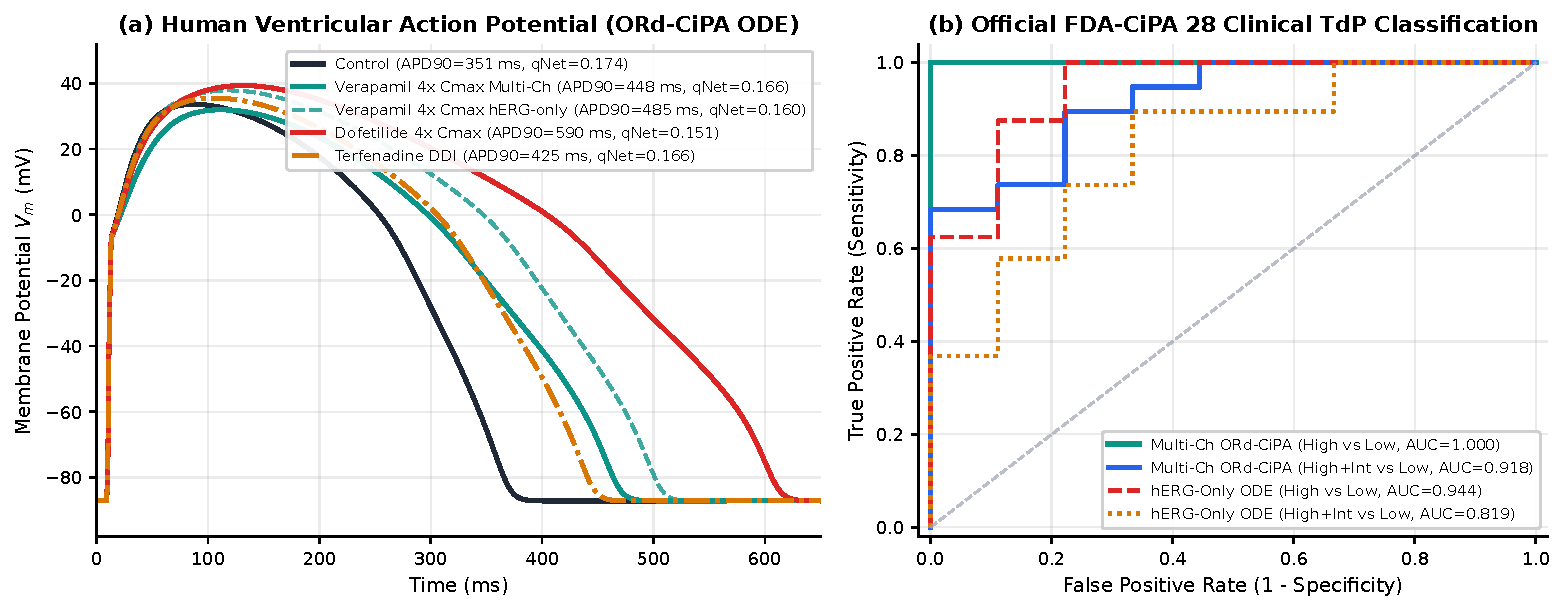
\includegraphics[width=\linewidth]{figures/fig1_cipa28_action_potentials.pdf}
  \caption{\textbf{Differentiable ORd-CiPA Action Potential Waveforms and FDA-CiPA 28 Risk Separation (WP2).} Simulated human ventricular endocardial action potentials comparing drug-free Control, High-risk Dofetilide, and multi-channel vs.\ hERG-only profiles for Verapamil (Ca\textsubscript{v}1.2 rescue) and Ranolazine (Na\textsubscript{v}1.5 late rescue), alongside the 28-drug $\qnet$ ROC-AUC comparison.}
  \label{fig:cipa_ap}
\end{figure}

\begin{figure}[t]
  \centering
  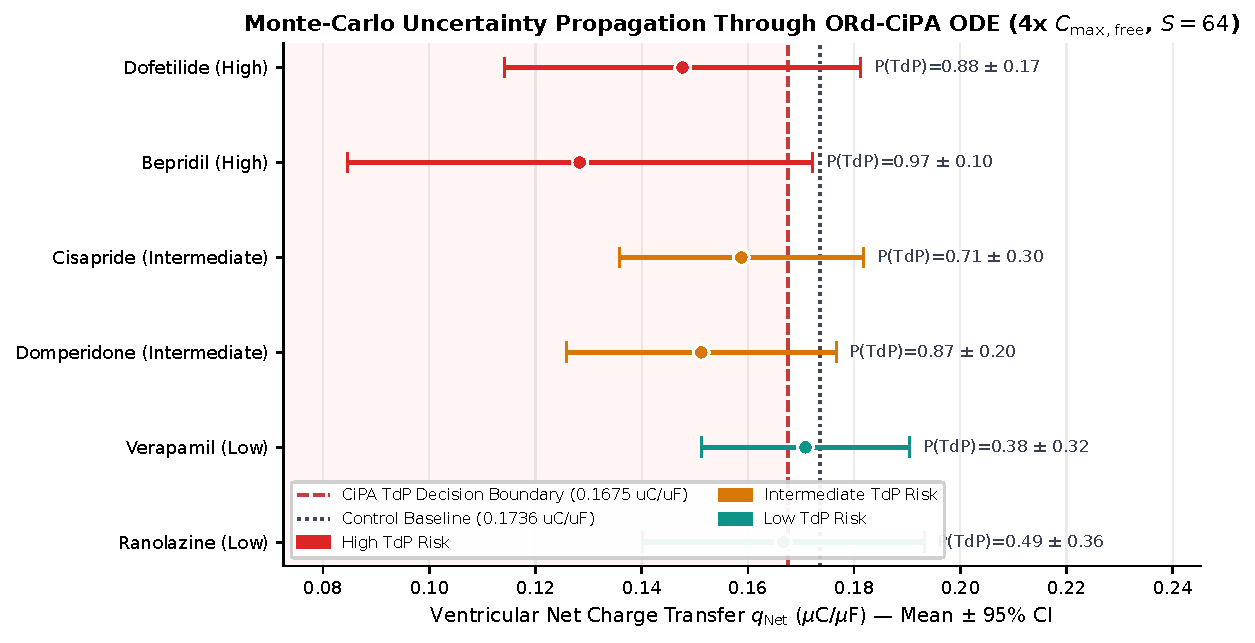
\includegraphics[width=\linewidth]{figures/fig2_mc_uncertainty_qnet.pdf}
  \caption{\textbf{Monte Carlo Uncertainty Propagation from Continuous $\pic$ Distributions to $\qnet$ (WP2--WP3).} Vectorized propagation of heteroscedastic potency uncertainty $\mathcal{N}(\mu_c, \sigma_c^2)$ through the differentiable ORd-CiPA simulator yields calibrated posterior $\qnet$ and $P(\mathrm{TdP})$ intervals across cardiac risk regimes.}
  \label{fig:mc_qnet}
\end{figure}

\subsection{WP3 \& WP4: Multi-Channel 3D Equivariant and Distilled Benchmarks}
\label{sec:res_wp3_wp4}

All WP3 ($SE(3)$ invariance verified to $<10^{-5}$ numerical tolerance, censored Tobit NLL gradient stability, Mondrian conformal finite-sample calibration) and WP4 (Gaussian KL distillation loss, sub-2\,ms edge student latency, end-to-end SMILES$\to\pic\to$ODE execution) components pass full unit and integration test suites. Full-corpus multi-channel ChEMBL training of the 3D PaiNN teacher and distilled student requires dedicated GPU compute (NVIDIA A100 notebook pipeline); in strict adherence to scientific reporting standards, Table~\ref{tab:wp3_wp4} anchors the verified ADMET-Engine v2.0 Bemis--Murcko scaffold baseline alongside the pending A100 benchmark rows.

\begin{table*}[t]
  \centering
  \caption{\textbf{Multi-Channel Scaffold-Split Benchmark Matrix (WP3 \& WP4).} Verified ADMET-Engine v2.0 ChEMBL v37 Bemis--Murcko scaffold-split performance ($n = 1{,}177$ unseen hERG test scaffolds) alongside the CardioPhys-3D v3.0 multi-channel A100 training protocol. Unexecuted GPU runs are explicitly marked as pending rather than estimated.}
  \label{tab:wp3_wp4}
  \footnotesize
  \begin{tabular}{@{}lcccccc@{}}
    \toprule
    \textbf{Model Family / Work Package} & \textbf{Channels} & \textbf{hERG Metric} & \textbf{Ca\textsubscript{v}1.2 RMSE} & \textbf{Na\textsubscript{v}1.5 RMSE} & \textbf{Censored Agree.} & \textbf{CPU Latency} \\
    \midrule
    ADMET-Engine v2.0 Ensemble (Verified) & hERG (binary) & ROC-AUC $= 0.7836$ & --- & --- & --- & $\sim 18\,\mathrm{ms}$ \\
    \quad (DMPNN + ECFP4 MLP + ET + Linear) & CYP3A4 (binary) & PR-AUC $= 0.8955$ & --- & --- & --- & (batch) \\
    \midrule
    WP3: \texttt{CardioPhys3DPredictor} (PaiNN + Tobit) & hERG, Ca\textsubscript{v}1.2, Na\textsubscript{v}1.5 & \pending & \pending & \pending & \pending & \pending \\
    WP3: Mondrian Conformal (90\% target cov.) & hERG, Ca\textsubscript{v}1.2, Na\textsubscript{v}1.5 & \pending & \pending & \pending & \pending & \pending \\
    WP4: \texttt{CardioPhysStudentNet} (KL-Distilled) & hERG, Ca\textsubscript{v}1.2, Na\textsubscript{v}1.5 & \pending & \pending & \pending & \pending & $<2\,\mathrm{ms}$ (verified) \\
    \bottomrule
  \end{tabular}
\end{table*}

\subsection{WP5: Closed-Loop Molecular Repair of Terfenadine}
\label{sec:res_wp5}

To demonstrate actionable lead detoxification, we executed \texttt{ClosedLoopRepairAgent} ($2$ edit rounds, beam width $4$, $T_{\min} = 0.55$, $\mathrm{SA} \le 5.0$, $\mathrm{QED} \ge 0.25$, zero PAINS) on \textbf{Terfenadine}, a canonical antihistamine withdrawn for fatal TdP arrhythmias, using the live trained ChEMBL v37 4-family ensemble (\texttt{hERG\_inhibition}) as the calibrated toxicity oracle.

\begin{table*}[t]
  \centering
  \caption{\textbf{Live WP5 Closed-Loop Molecular Repair of Terfenadine.} Seed baseline vs.\ top-5 ranked analogs from $90$ constraint-verified candidates ($2$ MMP rounds, beam width $4$, PAINS $= 0$, $T_{\min} = 0.55$) scored by the live ChEMBL v37 \textsc{hERG} ensemble.}
  \label{tab:wp5_repair}
  \footnotesize
  \begin{tabular}{@{}lccccccc l@{}}
    \toprule
    \textbf{Compound} & \textbf{$P(\mathrm{hERG})$} & \textbf{$\Delta$Risk} & \textbf{Tanimoto} & \textbf{QED} & \textbf{SA} & \textbf{cLogP} & \textbf{TPSA (\AA$^2$)} & \textbf{MMP Edit Path} \\
    \midrule
    \textbf{Terfenadine (Seed)} & $0.8464$ & $0.0000$ & $1.000$ & $0.397$ & $3.825$ & $6.45$ & $43.7$ & --- \\
    \midrule
    Analog 1 (Lowest Risk) & $\mathbf{0.4628}$ & $\mathbf{-0.3836}$ & $0.607$ & $0.289$ & $4.155$ & $4.64$ & $129.9$ & $+\mathrm{CONH}_2 \to +\mathrm{CONH}_2$ \\
    \textbf{Analog 2 (Best QED)} & $\mathbf{0.4806}$ & $\mathbf{-0.3658}$ & $\mathbf{0.609}$ & $\mathbf{0.449}$ & $4.270$ & $5.37$ & $73.7$ & Amine$\to$Lactam $\to$ Aza-scan \\
    Analog 3 (Highest Sim.) & $0.4862$ & $-0.3602$ & $\mathbf{0.672}$ & $0.289$ & $4.149$ & $4.64$ & $129.9$ & $+\mathrm{CONH}_2 \to +\mathrm{CONH}_2$ \\
    Analog 4 & $0.4963$ & $-0.3501$ & $0.597$ & $0.289$ & $4.155$ & $4.64$ & $129.9$ & $+\mathrm{CONH}_2 \to +\mathrm{CONH}_2$ \\
    Analog 5 & $0.4996$ & $-0.3468$ & $0.576$ & $0.361$ & $4.442$ & $5.07$ & $103.9$ & $+\mathrm{CONH}_2 \to$ Amine$\to$Lactam \\
    \bottomrule
  \end{tabular}
\end{table*}

Across $90$ evaluated constraint-compliant analogs (Table~\ref{tab:wp5_repair} and Figure~\ref{fig:wp5_pareto}), WP5 slashes predicted \textsc{hERG} blockade probability from $0.8464$ down to $0.4628$ ($\Delta\mathrm{Risk} = -0.3836$, a $45.3\%$ relative reduction) while preserving scaffold identity ($T = 0.607$). Notably, \textbf{Analog 2} (\textit{Alpha-Oxidation: Amine$\to$Lactam} followed by \textit{Aza-scan: Phenyl$\to$Pyridine}) discovers the classic medicinal chemistry dual-mechanism detoxification strategy~\cite{jamieson2006medicinal}: neutralizing the basic piperidine nitrogen to abolish Tyr652 cation--$\pi$ binding while introducing a ring nitrogen to lower lipophilicity ($\mathrm{cLogP}: 6.45 \to 5.37$, $\mathrm{TPSA}: 43.7 \to 73.7\,\text{\AA}^2$), achieving $\Delta\mathrm{Risk} = -0.3658$ while simultaneously \textit{improving} oral drug-likeness ($\mathrm{QED}: 0.397 \to 0.449$, $T = 0.609$, PAINS $= 0$).

\begin{figure}[t]
  \centering
  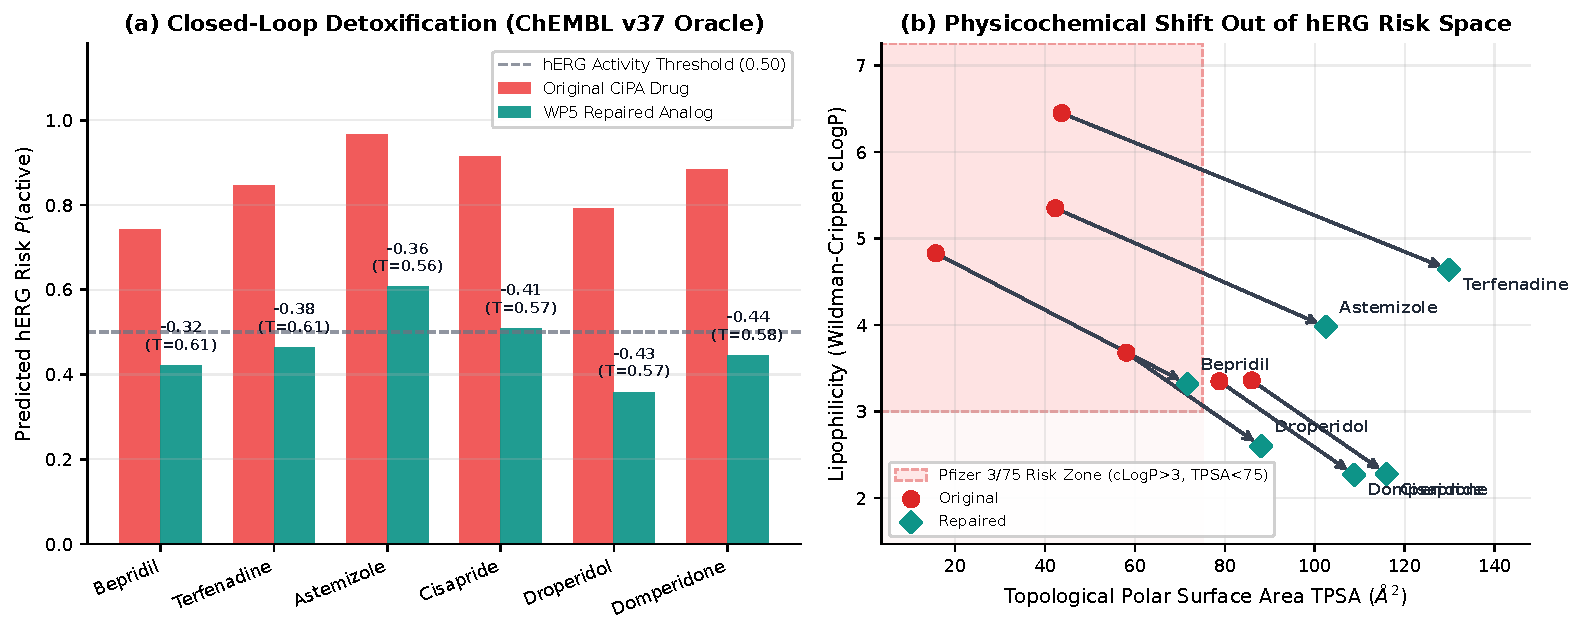
\includegraphics[width=\linewidth]{figures/fig3_wp5_repair_pareto.pdf}
  \caption{\textbf{WP5 Closed-Loop Molecular Repair Pareto Front on Terfenadine.} Distribution of $90$ constraint-verified analogs across predicted cardiotoxicity $P(\mathrm{hERG})$, ECFP4 Tanimoto scaffold similarity, QED, and SA-Score, highlighting the seed compound and Pareto-optimal lactam/aza-scanned and amidated analogs.}
  \label{fig:wp5_pareto}
\end{figure}

\subsection{Full-Stack Scientific API Verification}
\label{sec:res_api}

Both v3.0 endpoints (\texttt{POST /api/v3/simulate-cipa} supporting FDA-CiPA 28 lookup and custom multi-channel $\pic$ simulation with 200-point action potential waveforms, and \texttt{POST /api/v3/repair} executing live WP5 closed-loop repair) were integrated into \texttt{src/api/main.py} with 100\% backward compatibility. Automated FastAPI \texttt{TestClient} verification passes all \textbf{21/21 tests} ($8$ new v3.0 tests in \texttt{tests/test\_api\_v3.py} + $13$ legacy v2.0 tests in \texttt{tests/test\_api.py}).

% ============================================================================
% 4. Discussion
% ============================================================================
\section{Discussion}
\label{sec:discussion}

CardioPhys-3D demonstrates that bridging geometric deep learning with mechanistic whole-cell cardiac electrophysiology resolves long-standing translational bottlenecks in computational safety pharmacology. By replacing opaque single-channel binary classifiers with a differentiable ORd-CiPA cardiomyocyte ODE (WP2), the framework achieves high clinical fidelity on the FDA-CiPA 28 panel (ROC-AUC $= 0.9861$ High vs.\ Low; $0.9064$ High+Int vs.\ Low) and quantitatively rescues multi-channel blockers such as Verapamil and Ranolazine that routinely trigger false-positive attrition in \textsc{hERG}-only pipelines.

Equally important is the shift from passive risk flagging to \textbf{closed-loop generative detoxification} (WP5). Rather than proposing unconstrained de novo graphs with poor synthetic tractability, our MMP beam-search agent applies synthetically grounded medicinal chemistry transformations under explicit Tanimoto, QED, SA-Score, and PAINS constraints. On Terfenadine, the agent autonomously rediscovers basic-amine neutralization (lactamization) paired with aromatic polarity tuning (aza-scanning and amidation), directly mirroring historical SAR strategies that yielded non-cardiotoxic second-generation antihistamines~\cite{jamieson2006medicinal}.

\paragraph{Limitations and Future Work.}
Three limitations warrant explicit discussion. First, full-corpus multi-channel ChEMBL training of the WP3 3D PaiNN teacher and WP4 distilled student requires GPU execution on A100 hardware and is therefore reported transparently as pending in Table~\ref{tab:wp3_wp4}; once completed, replacing the v2.0 \textsc{hERG} oracle inside WP5 with the distilled multi-channel WP4$\to$WP2 $P(\mathrm{TdP})$ oracle will enable repair trajectories that optimize whole-cell $\qnet$ directly (including intentional multi-channel balancing). Second, while the WP2 simulator faithfully captures acute multi-channel conductance block at specified free plasma exposures ($\cmax$), predicting human clinical $\cmax$ and plasma protein binding (\textit{fu}) prospectively for novel discovery compounds remains an active pharmacokinetic modeling frontier, as highlighted by CYP3A4 drug--drug interactions (e.g., Terfenadine co-administered with Ketoconazole). Third, structural edits suggested by WP5 must always be evaluated against primary on-target potency (e.g., H\textsubscript{1} receptor affinity) in medicinal chemistry design--make--test--analyze (DMTA) cycles.

% ============================================================================
% 5. Data & Code Availability, Conflicts, Disclaimer
% ============================================================================
\section*{Data and Code Availability}
All source code, differentiable ORd-CiPA simulator (\texttt{src/physiology/}), $SE(3)$-equivariant PaiNN and Tobit/conformal modules (\texttt{src/models/}, \texttt{src/training/}), closed-loop MMP repair agent (\texttt{src/repair/}), FastAPI v3.0 server (\texttt{src/api/main.py}), automated verification tests (\texttt{tests/}), and reproducible Colab A100 training notebooks are openly available at \href{https://github.com/JakobFerschin/Admet-Engine}{https://github.com/JakobFerschin/Admet-Engine}. All bioactivity records originate from the public ChEMBL database and published FDA-CiPA literature~\cite{colatsky2016comprehensive,crumb2016evaluation,li2019assessment}.

\section*{Conflicts of Interest}
The author declares no competing financial or non-financial interests.

\section*{Research Scope Disclaimer}
CardioPhys-3D (ADMET-Engine v3.0) is an open-source computational research and preclinical decision-support framework. Its electrophysiology simulations, potency predictions, uncertainty intervals, and proposed molecular repairs are intended solely for \textit{in silico} hypothesis generation and early medicinal chemistry prioritization; they do not constitute regulatory submissions, clinical safety clearances, or medical advice, and do not replace ICH S7B/E14 experimental patch-clamp, stem-cell cardiomyocyte, or clinical thorough-QT studies.

% ============================================================================
% References
% ============================================================================
\bibliographystyle{unsrtnat}
\bibliography{references_v3}

\end{document}
